
\subsection{Detaillierte Vegetationsstruktur}

\subsubsection{Geltinger Bucht}

Die Vegetationsbestände in der Geltinger Bucht (dicht bewachsener Standort) setzen sich zusammen aus \textit{Zostera marina} und \textit{Fucus vesiculosus f. balticus}. Das Seegras wuchs bis \unit{30}{\centi\metre} vom Grund mit Deckungsgraden von \unit{70-80}{\%}. In den Wasserschichten darüber bis \unit{60}{\centi\metre} vom Grund reduzierte sich die Deckung allmählich bis auf \unit{10}{\%}. Nur wenige der schmalen Blattspreiten erstreckten sich darüber hinaus bis zur Oberfläche. Das Wasser war hier etwa \unit{100}{\centi\metre} tief.

Der lose Blasentang ist von kräftigem Wuchs und bedeckt den Boden mit \unit{20}{\%}. Auf \unit{20 und 30}{\centi\metre} Höhe gehen die Pflanzen in die Breite und sorgen für Deckungen von \unit{30}{\%}, darüber verschmälert sich der Blasentang wieder. Große Exemplare erreichten Wuchshöhen von bis zu \unit{50}{\centi\metre}.
In der Mitte der Wassersäule befanden sich mit Deckungsgraden unter einem Prozent freischwimmende filamentöse Algen, die jedoch an zwei Plots Deckungen von \unit{10 und 20}{\%} ausmachten. Die Gesamtdeckung auf den Flächen betrug \unit{90}{\%}, diese wurden vom Grund bis \unit{20}{\centi\metre} Wuchshöhe kartiert, danach nahmen die Deckungen stetig bis zur Oberfläche ab.

\subsubsection{Orther Bucht}

Die Orther Bucht ist zu \unit{30-60}{\%}, im Mittel mit \unit{40}{\%} mit Pflanzen bedeckt. Auf \unit{10}{\centi\metre} Entfernung vom Grund sind \unit{30}{\%} der Wasserschicht bedeckt, darüber ragen nur noch einzelne Stängel von \textit{Potamogeton pectinatus} bis \unit{40}{\centi\metre} Höhe. Das Wasser an diesem Standort ist im Mittel \unit{70}{\cm} tief. Bestandsbildende Art ist \textit{Zannichellia palustris} mit Deckungen von \unit{20-40}{\%}. An einem Plot fehlte die Art, dafür kam hier \textit{Ruppia cirrhosa} mit einer Deckung von \unit{40}{\%} vor. Ebenfalls deckten filamentöse Algen auf \unit{5 bis 10}{\centi\metre} Wuchshöhe zu \unit{20}{\%} den Standort ab. \textit{Potamogeton pectinatus} kam mit Deckungen von bis zu \unit{10}{\%} am Grund vor und verschmälerte sich in der Wassersäule. Von \textit{Chara canescens} und \textit{Tolypella nidifica} wurden vereinzelt Exemplare gefunden.

\subsubsection{Salzhaff}

Das Salzhaff ist zu \unit{80-90}{\%} mit Vegetation bedeckt. Davon machen nicht fest verankerte, filamentöse Algen mit \unit{80}{\%} Deckung auf \unit{5}{\centi\metre} Wuchshöhe den größten Anteil aus. Ihr Anteil reduziert sich in der Wassersäule allmählich bis auf \unit{50}{\centi\metre} Wuchshöhe. \textit{Potamogeton pectinatus} ist mit \unit{30-60}{\%} Deckung die bastandsbildene festsitzende Pflanzenart. Auch sein Anteil reduziert sich allmählich bis \unit{50}{\centi\metre} Wuchshöhe, darüber hinaus reichen wenige Äste bis zur Oberfläche. Das Wasser an diesem Standort ist \unit{80 bis 90}{\centi\metre} tief. Vereinzelt kam auch lose am Grund die Alge \textit{Monostroma sp}. und \textit{Zannichellia palustris} vor.

\subsubsection{Spandowerhagener Wiek}

Die gesamte Spandowerhagener Wiek war zu etwa \unit{90}{\%} mit Pflanzen bedeckt, es gab keine ausgedehnten freien Flächen. Den Hauptanteil der Vegetation bildete \textit{Potamogeton pectinatus} mit Deckungsgraden von im Mittel \unit{90}{\%} am Grund, sich allmählich in der Wassersäule reduzierend. Dabei trägt er auf \unit{30}{\centi\metre} Wuchshöhe noch zu einer mittleren Deckung von \unit{50}{\%} bei und wächst bis \unit{50}{\centi\metre} auf. Das Wasser ist \unit{80-85}{\centi\metre} tief. Außerdem kommen \textit{Myriophyllum spicatum} mit \unit{10 bis 20}{\%} Deckung und \textit{Potamogeton perfoliatus}, auf einigen Plots mit bis zu \unit{10}{\%} Deckung vor. \textit{Myriophyllum spicatum} bedeckt mit einem Grund-Abstand von \unit{10 und 20}{\centi\metre} noch \unit{10 bzw. 5}{\%} der jeweiligen Wasserschichten, nur vereinzelte Halme wachsen bis \unit{50}{\centi\metre} auf. \textit{Potamogeton perfoliatus} hingegen nimmt nur bis auf \unit{10}{\centi\metre} relevante Deckungen ein, darüber hinaus gehen wenige Zweige bis \unit{70}{\centi\metre} Wuchshöhe. Auf 2 Plots wurde auch mit \unit{10 bzw. 20}{\%} Anteil in der Wasserschicht \textit{Zannichellia palustris} gefunden und es gab wenige vereinzelte Exemplare von \textit{Najas marina}.





\begin{figure}[htb]
\centering
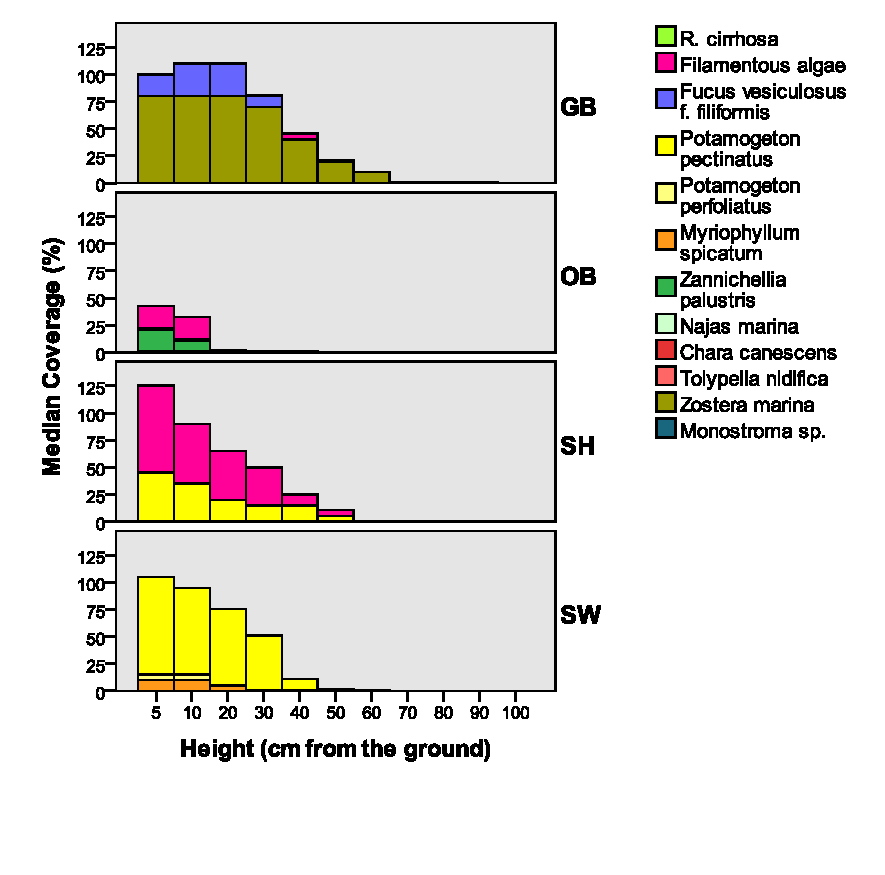
\includegraphics[0.90\textwidth]{images/Wuchshoehenkartierung/salzgradient_gross1.eps}
\caption[Höhenstufenkartierung an den Stationen des Salzgradienten (+M)]{Deckungen aller Arten auf Höhenstufen vom Grund bis zur Oberfläche an den dicht bewachsenen Standorten entlang des Salzgradienten; GB = Geltinger Bucht, OB = Orther Bucht; SH = Salzhaff; SW = Spandowerhagener Wiek}
\label{fig:wuchshoehen_salzgradient_1}
\end{figure}
\\
\begin{figure}[htb]
\centering
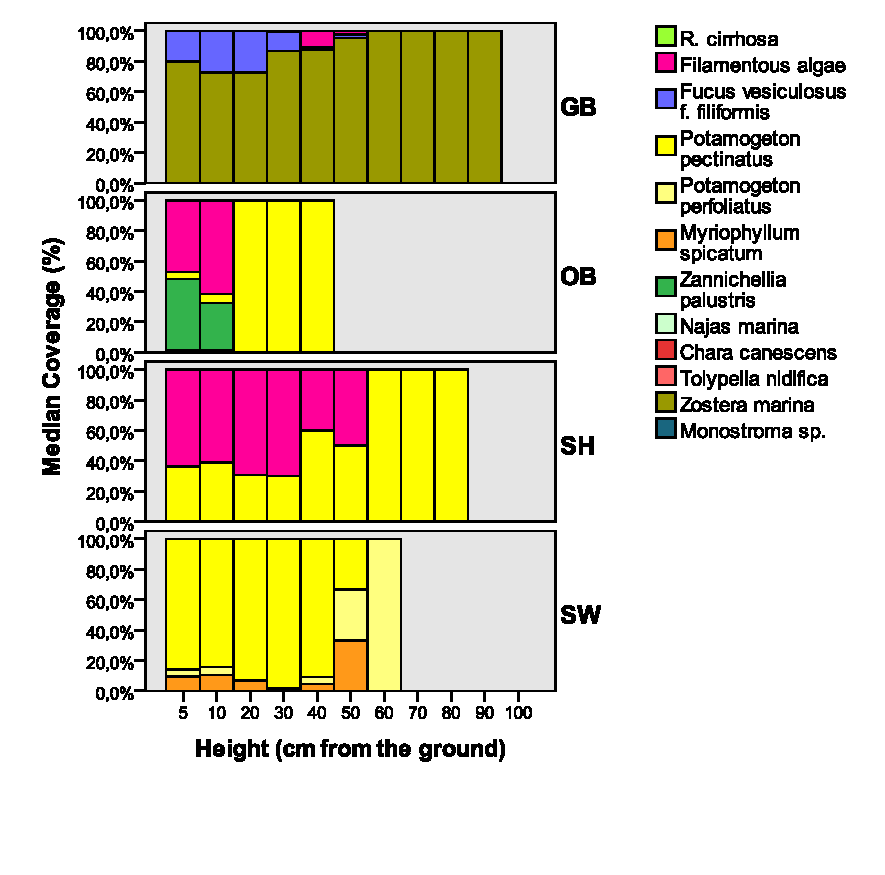
\includegraphics[0.90\textwidth]{images/Wuchshoehenkartierung/salzgradient_gross2.eps}
\caption[Prozentuale Höhenstufenkartierung an den Stationen des Salzgradienten (+M)]{Prozentuale Deckungen aller Arten, bezogen auf die Gesamtdeckung auf jeder Höhenstufe an den dicht bewachsenen Standorten entlang des Salzgradienten; GB = Geltinger Bucht, OB = Orther Bucht; SH = Salzhaff; SW = Spandowerhagener Wiek}
\label{fig:wuchshoehen_salzgradient_2}
\end{figure}

\FloatBarrier


\subsection{Deckung und PVI}

Zum Zeitpunkt der Probenahmen entlang des Salzgradienten waren sowohl die Deckung als auch das PVI an allen vegetationsarmen Untersuchungsgruppen sehr gering. Maximal 2 \unit{2}{\%} der Fläche wurden von Phytobenthos eingenommen und es machte maximal \unit{0,3}{\%} der Wassersäulen aus.

Bei Betrachtung aller vegetationsdominierten Stationen des Salzgradienten im Vergleich zeigt sich, dass es 3 verschiedene Kategorien von Vegetationsbeständen gab. In die erste Kategorie fallen die Orther Bucht und die Griebener Bucht. Diese zeigten Deckungsgrade von \unit{40-60}{\%} Auch ihre pflanzliche Zusammensetzung ist sich ähnlich. Es gibt grundrasenbildende Arten (\textit{Zannichellia palustris} in der Orther Bucht und\textit{ Ruppia cirrhosa} in der Griebener Bucht) sowie das höher aufwachsende Laichkraut \textit{Potamogeton pectintus} und dazwischen Matten aus fädigen Algen. In dem verhältnismäßig flachen Wasser von \unit{60-70}{\centi\metre} werden PVI-Werte von im Mittel \unit{5}{\%} erreicht. Das Maximum waren \unit{14,4}{\%} in der Orther Bucht.

Die Geltinger Bucht, das Salzhaff und die Spandowerhagener Wiek bilden die zweite Kategorie mit wesentlich höheren Deckungsgraden von \unit{80-95}{\%} und ebenfalls hohen PVI-Werten von \unit{20-30}{\%}. Diese Standorte befinden sich auch in etwas tieferem Wasser (\unit{80-110}{\centi\metre}. Die Geltinger Bucht und die Spandowerhagener Wiek sind sich auch in ihrer Vegetationsstruktur ähnlich. Beide beherbergen Makrophyten, die weit in die Wassersäule hineinreichen und auch in größerem Abstand vom Grund noch hohe Deckungsgrade verursachen. In der Geltinger Bucht ist dies \textit{Zostera marina} und in der Spandowerhagener Wiek sind es parvopotamiden und Myriophyllum spicatum. Im Salhhaff hingegen werden die hohen Deckungsgrade und pflanzlichen Anteile in der Wassersäule neben dem hoch aufwachsenden \textit{Potamogeton pectintus} zu einem großen Teil von filamentösen Algen verursacht.

Die dritte Kategorie nimmt der Vitter Bodden ein. Bei einer Bedeckung von \unit{100}{\%} ist der Anteil des Phytobenthos an der Wassersäule mit \unit{8-17}{\%} deutlich weniger als bei den 3 zuvor genannten Standorten. Grund hierfür ist die dichte Bedeckung mit \textit{Fucus vesiculosus}, welcher zwar hohe Deckungsgrade verursacht, aber nicht weit in die etwa \unit{83}{\centi\metre} tiefe Wassersäule hineinreicht.



\begin{figure}[htb]
\centering
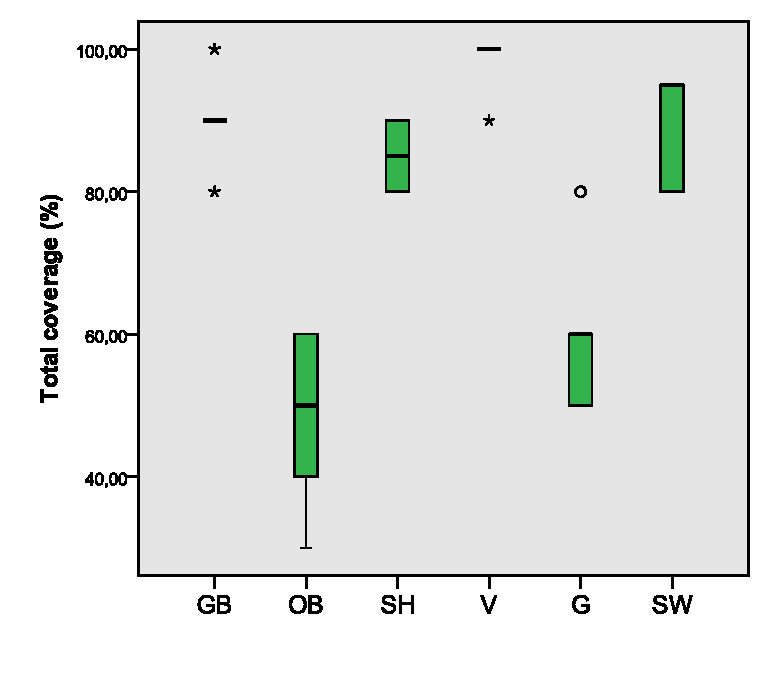
\includegraphics[width=0.80\textwidth]{images/total_cover/cover_salzgradient.eps}
\caption[Bedeckung mit Makrophyten an Standorten entlang des Salzgradienten]{Gesamtbedeckung der Plots mit Makrophyten an den dicht bewachsenen Standorten entlang des Salzgradienten; GB = Geltinger Bucht, OB = Orther Bucht; SH = Salzhaff; SW = Spandowerhagener Wiek}
\label{fig:cover_salzgradient}
\end{figure}

\begin{figure}[htb]
\centering
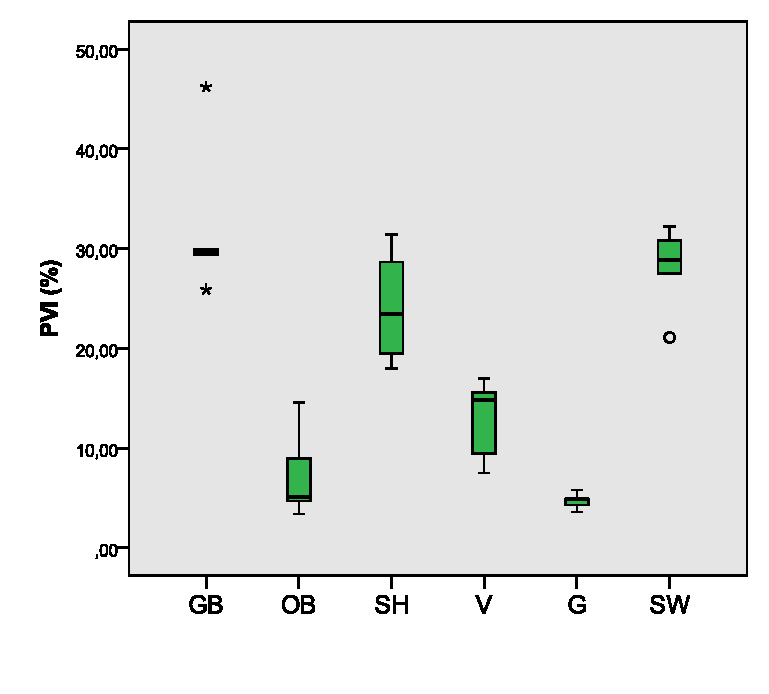
\includegraphics[width=0.80\textwidth]{images/pvi/pvi_salzgradient.eps}
\caption[PVI an Standorten entlang des Salzgradienten]{Anteil des Phytobenthos an der Wassersäule (PVI nach \cite{jeppesen_1998}) an den dicht bewachsenen Standorten entlang des Salzgradienten; GB = Geltinger Bucht, OB = Orther Bucht; SH = Salzhaff; SW = Spandowerhagener Wiek}
\label{fig:pvi_salzgradient}
\end{figure}



\begin{table}[!htb]
\centering
\caption[Deskriptive Statistik, Deckung und PVI entlang des Salzgradienten]{Deskriptive Statistik zu Deckung und PVI an Standorten entlang des Salzgradienten; MAD = Mittlere Abweichung vom Median}
\begin{tabular}{llllll}
\toprule
Category & Location 							& \multicolumn{2}{l}{Total Cover} & \multicolumn{2}{l}{PVI}\\
		 &											& Median	& MAD			  & Median	& MAD\\
\midrule
\multirow{6}{*}{Dense Vegetation}& Geltinger Bucht	& 90.00		& 4.00			  & 29.60	& 4.16\\
								 & Orther Bucht		& 50.00		& 10.00			  & 5.10	& 3.10\\
								 & Salzhaff			& 85.00		& 5.00			  & 23.35	& 4.58\\
								 & Vitter Bodden	& 100.00	& 2.00			  & 14.80	& 3.12\\
								 & Griebener Bucht	& 60.00		& 8.00			  & 4.90	& 0.56\\
								 & Spandowerhagener Wiek & 95.00 & 6.00			  & 28.90	& 2.88\\
\midrule
\multirow{5}{*}{Sparse Vegetation}&Geltinger Bucht	& 2.00		& 0.00			  & 0.18	& 0.00\\
								 & Orther Bucht		& 2.00		& 				  & 0.30\\
								 & Salzhaff			& 0.50		& 0.00			  & 0.10	& 0.00\\
								 & Vitter Bodden	& 0.50		& 0.00			  & 0.00	& 0.00\\
								 & Griebener Bucht	& 2.50		& 1.30			  & 0.33	& 0.01\\
\bottomrule
\end{tabular}
\label{tab:statistik_salzgradient_Deckung,PVI}
\end{table}



\subsection{Sediment}

\subsubsection{Geltinger Bucht}

Das Sediment am dicht mit Phytobenthos besiedelten Standort ist mäßig sortiert und die Verteilungskurve etwas in den grobkörnigen Bereich verschoben. Feinsand und Mittelsand haben mit \unit{45 und 27,5}{\%} den größten Anteil am Gesamt-Korngrößenspektrum. Mit \unit{9 und 8,3}{\%} sind auch sehr grobe und grobe Sande im Sediment enthalten und mit je etwa \unit{5}{\%} sind Feinsand und Ton-/Siltfraktionen vertreten. Der Median der Korngrößenverteilung beträgt \unit{2,2 $ \phi $}{\%} und der organische Gehalt \unit{1,4}{\%}.

Das Sediment der kaum mit Phytobenthos besiedelten Untersuchungsgruppe war besser sortiert als die der dicht besiedelten Gruppe. Feinsande und Mittelsande hatten hier einen größeren Anteil von \unit{53 und 34}{\%}. Sehr grober Sand war fast nicht und grober Sand nur zu \unit{3}{\%} enthalten. Es waren weniger feine Sande (\unit{2,5}{\%}) aber dafür mit etwa \unit{7}{\%} mehr Ton und Silt enthalten. Der Organische Gehalt ist mit \unit{0,7}{\%} geringer als bei den Sedimenten der dicht mit Seegras und \textit{Fucus} besiedelten Fläche.



\subsubsection{Orther Bucht}

Auf der Phytobenthos-dominierten Untersuchungsfläche ist das Sediment sehr gut sortiert und die Feinsandfraktion dominiert mit \unit{72}{\%}. Daneben kommen zu \unit{16 und 7}{\%} sehr feine und Mittelsande vor. Der Anteil der \unit{<63}{\mu\metre}-Fraktion beträgt hier nur \unit{3}{\%}. Insgesamt ist die Verteilungskurve leicht linksschief (in den feinkörnigen Bereich verschoben) und der Median der Korngröße beträgt \unit{1,6}{$ \phi $}. Der organische Gehalt des Sedimentes ist mit \unit{0,5}{\%} sehr gering.

Das Sediment der Vegetationsreichen Untersuchungsgruppe hingegen ist weniger gut sortiert. Mit \unit{62}{\%} ist der Feinsand ebenfalls die am meißten vertretene Korngrößenfraktion, jedoch ist auch der Anteil des Mittelsandes mit etwa \unit{18}{\%} höher. Der Median der Korngröße beträgt \unit{1,8}{$ \phi $} 

\subsubsection{Salzhaff}
\subsubsection{Spandowerhagener Wiek}



\begin{figure}[htb]
\centering
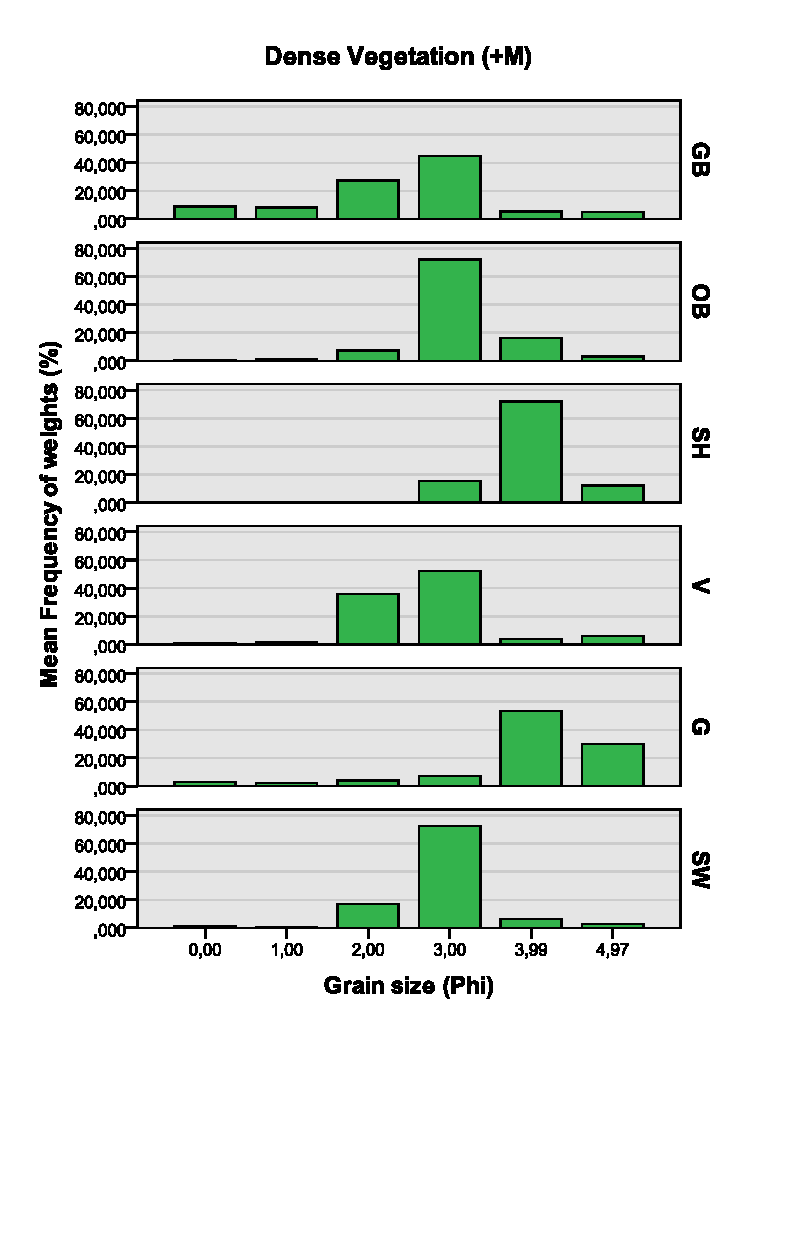
\includegraphics[trim = 0mm 25mm 0mm 0mm, clip, 0.90\textwidth]{images/grainsize/grain_size_big1.eps}
\caption[Korngrößenverteilungen entlang des Salzgradienten (+M)]{Korngrößenverteilungen an dicht bewachsenen Standorten entlang des Salzgradienten (+M); GB = Geltinger Bucht, OB = Orther Bucht; SH = Salzhaff; V = Vitter Bodden (5.7.2013), G = Griebener Bucht (30.7.2013), SW = Spandowerhagener Wiek}
\label{fig:korngrössen_salzgradient_+m}
\end{figure}

\begin{figure}[htb]
\centering
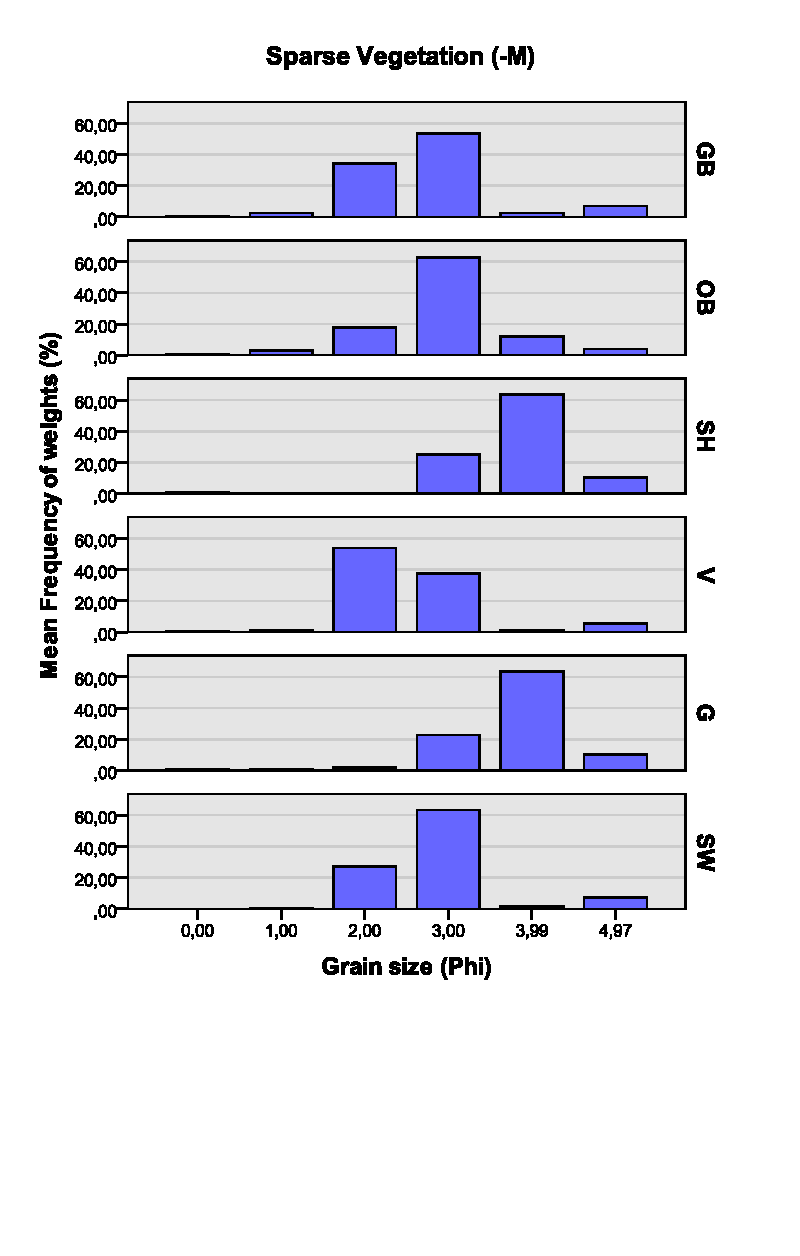
\includegraphics[trim = 0mm 25mm 0mm 0mm, clip, 0.90\textwidth]{images/grainsize/grain_size_big21.eps}
\caption[Korngrößenverteilungen entlang des Salzgradienten (-M)]{Korngrößenverteilungen an spärlich bewachsenen Standorten entlang des Salzgradienten (-M); GB = Geltinger Bucht, OB = Orther Bucht; SH = Salzhaff; V = Vitter Bodden (5.7.2013), G = Griebener Bucht (30.7.2013), SW = Spandowerhagener Wiek}
\label{fig:korngrössen_salzgradient_-m}
\end{figure}

\FloatBarrier



\begin{table}[!htb]
\centering
\caption[Deskriptive Statistik zu den Korngrößenverteilungen entlang des Salzgradienten]{Deskriptive Statistik zu den Korngrößenverteilungen an den Standorten entlang des Salzgradienten; MAD = Mittlere Abweichung vom Median; +M = dichte Vegetation, -M = spärliche Vegetation; Kennwerte aus den obersten \unit{2}{\centi\metre} des Sedimentkörpers}
\begin{tabular}{lcrrrr}

\toprule

\multicolumn{1}{c}{Location}  & \multicolumn{1}{c}{Category} & \multicolumn{1}{c}{Med Grain Size} & \multicolumn{1}{c}{Sorting} & \multicolumn{1}{c}{< \unit{63}{\mu\metre}} & \multicolumn{1}{c}{AFDW}\\

& \multicolumn{1}{c}{(mm)}	& \multicolumn{1}{c}{$ (\phi) $} & & \multicolumn{1}{c}{(\%)} & \multicolumn{1}{c}{(\%)}\\

\midrule
\multirow{2}{*}{Geltinger Bucht} & +M & 2.12 & 0.71 & 4.94 & 1.42\\
								 & -M & 2.24 & 0.54 & 6.88 & 0.72\\
\midrule
\multirow{2}{*}{Orther Bucht} & +M  & 2.57 & 0.35 & 3.03 & 0.52\\
							& -M  & 2.46 & 0.41 & 4.00 & 0.55\\
\midrule
\multirow{2}{*}{Salzhaff} & +M & 3.47 & 0.35 & 12.15 & 1.21\\
						& -M & 3.37 & 0.40 & 10.45 & 0.78\\
\midrule
\multirow{2}{*}{Vitter Bodden} & +M & 2.23 & 0.54 & 6.04 & 1.23\\
								& -M & 1.89 & 0.56 & 5.56 & 0.91\\
\midrule
\multirow{2}{*}{Griebener Bucht} & +M & 3.61 & 0.95 & 28.31 & 4.19\\
								& -M & 3.42 & 0.67 & 10.23 & 1.43\\
\midrule
\multirow{2}{*}{Spandowerhagener Wiek} & +M & 2.44 & 0.36 & 2.84 & 0.93\\
										& -M & 2.35 & 0.43 & 7.31 & 1.24\\

\bottomrule

\end{tabular}
\label{tab:statistik_salzgradient_sedimentparameter}
\end{table}


